\subsection{\citetitle{art_wu2019interior}}

\cite{art_wu2019interior} publicaron el artículo  \citetitle{art_wu2019interior} para la <<Association for Computing Machinery>> en el 2019.

Se presenta una técnica novedosa para la generación automática de planos de planta para edificaciones residenciales mediante un enfoque basado en datos. Este método se inspira en el proceso de diseño humano y ha demostrado un rendimiento superior en comparación con los métodos existentes. La generación automatizada de planos de planta es fundamental en el diseño de interiores, y esta investigación ofrece una perspectiva innovadora para abordar este desafío.

La metodología propuesta en este estudio se basa en un enfoque de dos etapas para la generación de planos de planta. En la primera etapa, se localizan las habitaciones, mientras que en la segunda etapa se definen las paredes interiores. Para entrenar eficazmente las redes neuronales utilizadas en este proceso, se presenta un conjunto de datos a gran escala denominado RPLAN, que contiene más de 80,000 planos de planta de edificaciones residenciales reales con habitaciones y paredes etiquetadas. Esta metodología imita el proceso creativo de los artistas humanos y ha demostrado ser efectiva en la generación automatizada de planos de planta. Para un ejemplo más claro se puede observar la Figura 3.

\begin{figure}[!ht]
	\begin{center}
		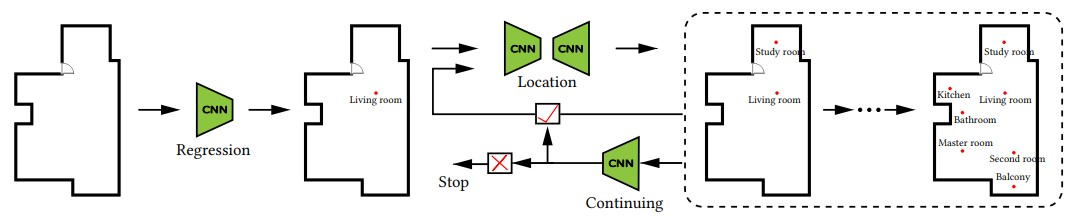
\includegraphics[width=1\textwidth]{2/figures/wu2019.jpg}
		\caption[Un modelo de predicción iterativo para predecir la ubicación de las habitaciones]{Un modelo de predicción iterativo para predecir la ubicación de las habitaciones.\\
			Fuente: \cite{art_wu2019interior}. \citetitle{art_wu2019interior}. (p. 4)}
		\label{2:fig111}
	\end{center}
\end{figure}

En cuanto al rendimiento, el modelo de regresión muestra un buen desempeño con un error promedio de 0.82 metros en el conjunto de validación, mientras que la red de continuación alcanza alrededor del 99\% de precisión en la validación. En la tarea de clasificación de píxeles, se enfrentan problemas de desequilibrio de clases, los cuales se solucionan mediante el uso de una pérdida cruzada ponderada. En cuanto a la generación de un plano vectorizado, el proceso toma aproximadamente cuatro segundos a partir de los límites del edificio como entrada.

\subsection{\citetitle{pr_ketkhaw2019deepl}}
\cite{pr_ketkhaw2019deepl}  publicaron la investigación \citetitle{pr_ketkhaw2019deepl}, en español "Predicción de la ubicación de puntos de acceso no autorizados basada en redes neuronales profundas", se publicó en el journal tailandés <<Journal of Mobile Multimedia>> en 2022.

El objetivo del estudio es desarrollar un método llamado LPRAP que utiliza redes neuronales profundas para predecir la ubicación de puntos de acceso no autorizados en redes inalámbricas locales. La detección y localización precisa de estos RAPs es esencial para garantizar la seguridad de las redes y proteger la información confidencial de posibles amenazas. El artículo no especifica el uso de una base de datos concreta. No obstante, detalla el procedimiento de preparación del conjunto de datos empleado para entrenar y evaluar su esquema de predicción de la ubicación de puntos de acceso no autorizados (RAP). Este procedimiento incluye la recopilación de indicadores de intensidad de señal recibida (RSSI) en distintas áreas de una red experimental. La recopilación de datos se lleva a cabo mediante la medición de la RSSI en diversas subáreas dentro de una red configurada, capturando un total de 900,000 marcos de balizas para los procesos de entrenamiento y prueba.

Los dos mecanismos principales del proceso LPRAP son la detección de RAPs y la predicción de su ubicación. Para determinar la intensidad de la señal recibida (RSSI) en cada subárea, se recopila un conjunto de marcos de balizas en la detección de RAP. Posteriormente, se clasifica la ubicación de los RAPs utilizando un espacio de características de 81 dimensiones. En cuanto a la predicción de ubicación, se utiliza la precisión de la predicción de ubicación para evaluar el rendimiento del esquema propuesto comparándolo con otros algoritmos de aprendizaje automático como SVM, KNN, Naive Bayes y MLP.

Los resultados del experimento muestran que LPRAP supera a todos los demás algoritmos de aprendizaje automático evaluados. La precisión de la predicción de la ubicación de los RAPs aumenta significativamente con el aumento del número de subáreas. Por ejemplo, LPRAP logra una precisión de predicción del 88,31\% para 3 subáreas, lo que demuestra su capacidad para detectar y encontrar RAPs en entornos de redes inalámbricas como se puede observar en la Figura 6.

\begin{figure}[!ht]
	\begin{center}
		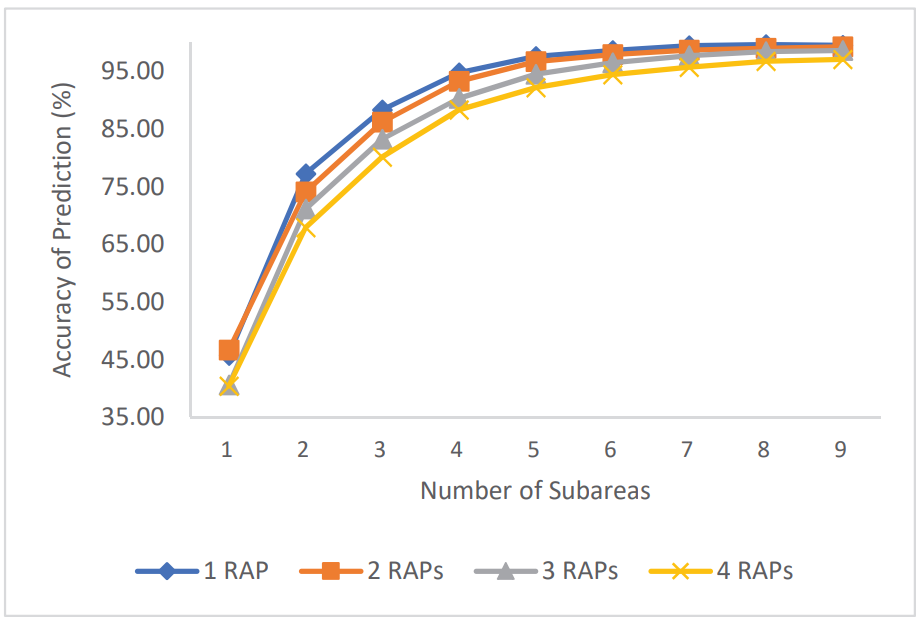
\includegraphics[width=0.75\textwidth]{2/figures/ketkha2022.png}
		\caption[Precisión de la predicción en función del número de subzonas para la predicción de la ubicación de 1 a 4 RAP.]{Precisión de la predicción en función del número de subzonas para la predicción de la ubicación de 1 a 4 RAP.\\
		Fuente: \cite{pr_ketkhaw2019deepl}. \citetitle{pr_ketkhaw2019deepl}. (p. 13)}
		\label{2:fig114}
	\end{center}
\end{figure}

\subsection{\citetitle{pr_nauata2021housegan}}
\cite{pr_nauata2021housegan} ,en la conferencia <<2021 IEEE/CVF Conference on Computer Vision and Pattern Recognition (CVPR)>>, que tuvo lugar en Nashville, Tennessee, Estados Unidos en el año 2021, publicaron un artículo titulado \citetitle{pr_nauata2021housegan}, en español se traduce como "House-GAN++: Generative Adversarial Layout Refinement Network hacia un agente computacional inteligente para arquitectos profesionales".

Para la generaci\'on automatizada de planos de planta, se sugiere una red generativa rival de refinamiento de dise\~no de planos de planta (House-GAN++). El sistema recibe un diagrama de burbujas que muestra las conexiones funcionales entre las habitaciones y, como salida, crea un plano de planta realista. El art\'iculo utiliza la base de datos RPLAN. Esta base de datos contiene 60,000 planos de casas en formato vectorial dise\~nados por arquitectos profesionales.

Como se muestra en la Figura 7, la arquitectura sugerida integra una GAN relacional con restricciones de grafo y una GAN condicional. El generador itera el diseño antes de convertirlo en la siguiente restricción de entrada. Cada componente recibe una máscara de segmentación de la verdad fundamental con una probabilidad aleatoria durante el entrenamiento (condicionamiento GT por componente).

\begin{figure}[!ht]
	\begin{center}
		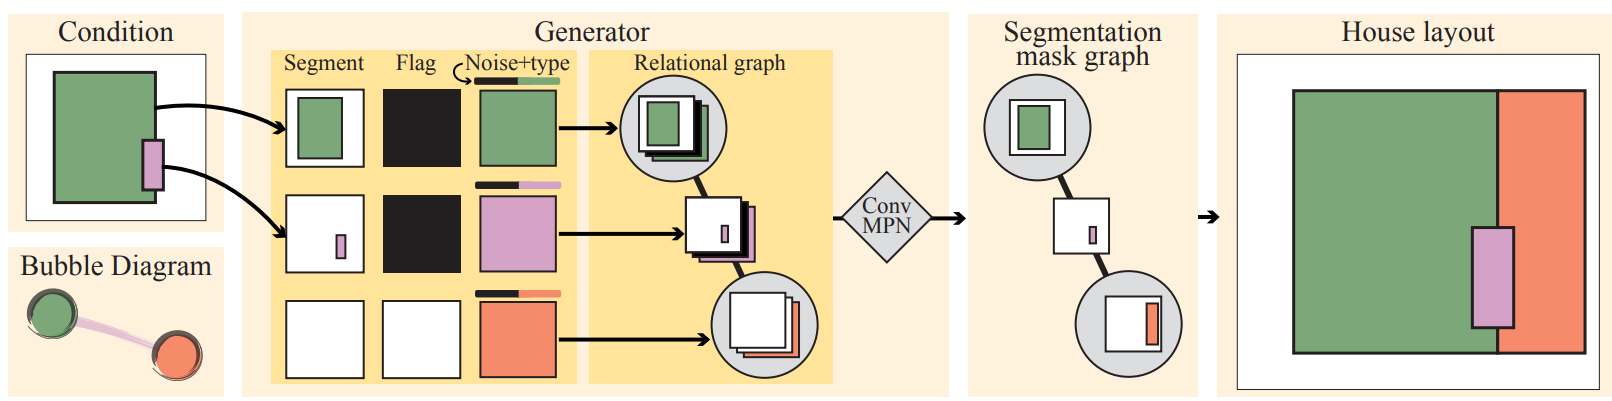
\includegraphics[width=0.8\textwidth]{2/figures/nauata2021.png}
		\caption[La arquitectura se basa en un GAN relacional. Se puede especificar una máscara de segmentación 2D adicional para cada habitación/puerta como condición de entrada, lo que permite un refinamiento iterativo del diseño.]{La arquitectura se basa en un GAN relacional. Se puede especificar una máscara de segmentación 2D adicional para cada habitación/puerta como condición de entrada, lo que permite un refinamiento iterativo del diseño.\\
		Fuente: \cite{pr_nauata2021housegan}. \citetitle{pr_nauata2021housegan}. (p. 3)}
		\label{2:fig115}
	\end{center}
\end{figure}

El sistema sugerido supera ampliamente los enfoques del estado del arte actuales en las tres métricas estándar de realismo, diversidad y compatibilidad. En un estudio de usuarios con arquitectos profesionales, el sistema obtuvo puntajes de realismo de -0.7 para los métodos comparativos y puntajes de 0.5 para el sistema propuesto en la tarea más difícil de generar planos de 8 habitaciones. Como se muestra en la Figura 8, la distancia de edición de gráficos (compatibilidad) aumenta de 11.8 para el estado del arte a 6.5 para el sistema propuesto en planos de 8 habitaciones.

\begin{figure}[!ht]
	\begin{center}
		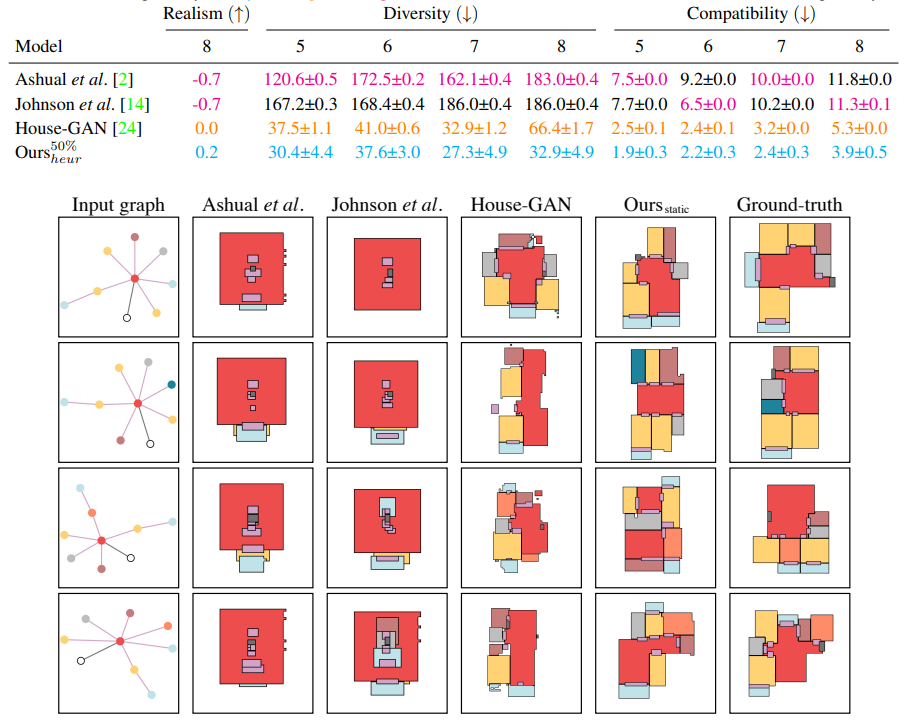
\includegraphics[width=1.1\textwidth]{2/figures/nauata2021_2.png}
		\caption[Evaluación del realismo. Se muestra un diseño generado para cada diagrama de burbujas de entrada]{Evaluación del realismo. Se muestra un diseño generado para cada diagrama de burbujas de entrada.\\
			Fuente: \cite{pr_nauata2021housegan}. \citetitle{pr_nauata2021housegan}. (p. 6)}
		\label{2:fig116}
	\end{center}
\end{figure}

\subsection{\citetitle{pr_cai2023precisewifi}}
\cite{pr_cai2023precisewifi} publicaron un artículo que se llamaba \citetitle{pr_cai2023precisewifi}, el término se traduce al español como "Posicionamiento WiFi preciso en el interior mediante algoritmos de aprendizaje profundo" para la revista científica <<ArXiv:2307.02011v>> publicada en 2023.

Este artículo presenta una nueva estrategia para el posicionamiento en interiores que emplea tecnología WiFi. Para mejorar la precisión del posicionamiento en comparación con el enfoque tradicional basado únicamente en RSSI, se recomienda utilizar una combinación de mediciones de la Intensidad de la Señal Recibida (RSSI) y el Ángulo de Llegada (AoA). En lugar de utilizar una base de datos predefinida, los autores realizaron sus propios experimentos en tres entornos interiores diferentes: un aula grande, un pasillo y un aula pequeña. Los datos para el estudio fueron recolectados directamente en estos entornos utilizando equipos WiFi y otros dispositivos de medición. El artículo se enfoca en la recolección de datos de Received Signal Strength Indicator (RSSI) y Angle of Arrival (AoA) en estos entornos para realizar el posicionamiento en interiores.

La metodología se compone de tres pasos principales: 1) Usando puntos de referencia, crear modelos de posicionamiento basados en RSSI y el método híbrido RSSI-AoA; 2) Entrenar los modelos utilizando varios algoritmos de aprendizaje profundo, como BPNN, RBF y CNN; 3) Probar el rendimiento de los modelos y calcular los errores en tres entornos de prueba diferentes: un salón de clases grande, un salón de clases pequeño y un salón de clases pasillo.

Independientemente del algoritmo de aprendizaje profundo utilizado y del entorno de prueba, los resultados muestran que el método híbrido RSSI-AoA tiene un error medio absoluto (MAE) más pequeño que el método basado únicamente en RSSI. Por ejemplo, el MAE del método híbrido con CNN es inferior a 300 mm en un salón de clases grande, mientras que el MAE del método basado en RSSI con CNN es inferior a 400 mm. Como se muestra en la Figura 9, el algoritmo CNN supera a BPNN y RBF en ambos modelos de posicionamiento.

\begin{figure}[!ht]
	\begin{center}
		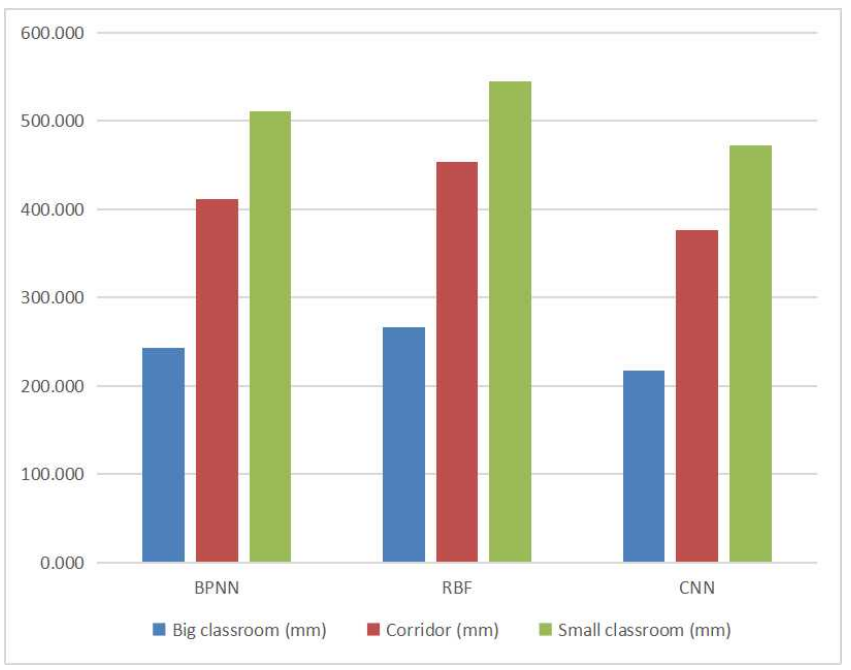
\includegraphics[width=0.90\textwidth]{2/figures/cai2023.png}
		\caption[Los MAE del modelo híbrido de posicionamiento]{Los MAE del modelo híbrido de posicionamiento.\\
			Fuente: \cite{pr_cai2023precisewifi}. \citetitle{pr_cai2023precisewifi}. (p. 26)}
		\label{2:fig117}
	\end{center}
\end{figure}

\subsection{\citetitle{pr_hosseini2023NSGAIIap}}
En el año 2023, la revista <<Automation in Construction>> publicó \cite{pr_hosseini2023NSGAIIap} publicaron el artículo conocido como \citetitle{pr_hosseini2023NSGAIIap}, "Ubicación óptima de puntos de acceso Wi-Fi basada en NSGA-II para posicionamiento interior: una predicción RSS basada en BIM", según su traducción al español.

Este artículo presenta un método para optimizar la colocación de puntos de acceso Wi-Fi (AP) en interiores utilizando un modelo de propagación de señal calibrado y un algoritmo genético multiobjetivo (NSGA-II), el cual codifica las posiciones de los APs en cromosomas binarios y aplica operadores genéticos para encontrar un conjunto de soluciones óptimas que minimizan el número de APs y maximizan la calidad del fingerprinting, considerando las restricciones del modelo BIM. El artículo no menciona la utilización de una base de datos externa. Los datos empleados parecen ser resultado de mediciones de campo realizadas por los autores dentro del edificio modelado en BIM.

La técnica consta de varias etapas: 1) Voxelización del modelo BIM del edificio, 2) Muestreo de intensidad de señal recibida (RSS) en puntos de control y verificación, 3) Calibrar el modelo de propagación de señal mediante el método de cuadrados mínimos, 4) Creación de huellas digitales virtuales 3D y 5) Uso de NSGA-II para optimizar la ubicación de los AP Wi-Fi. 

Los resultados demuestran que el método sugerido puede reducir significativamente el número de AP Wi-Fi necesarios sin sacrificar la precisión de la ubicación. La mejor solución encontrada tenía 4 APs y 13 APs, respectivamente, con una mejora en la precisión del posicionamiento del 35.54\% y 44.82\% en comparación con la distribución actual de 6 APs, como se muestra en la Figura 10.

\begin{figure}[!ht]
	\begin{center}
		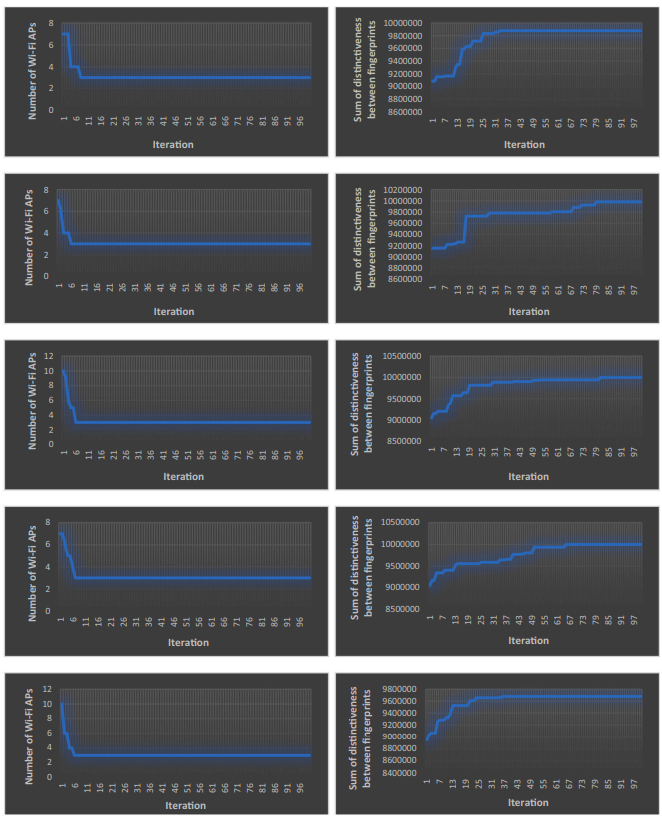
\includegraphics[width=0.75\textwidth]{2/figures/hosseini2023.png}
		\caption[Los resultados de la evaluación de la convergencia del NSGA-II]{Los resultados de la evaluación de la convergencia del NSGA-II.\\
		Fuente: \cite{pr_hosseini2023NSGAIIap}. \citetitle{pr_hosseini2023NSGAIIap}. (p. 16)}
		\label{2:fig118}
	\end{center}
\end{figure}

\subsection{\citetitle{pr_lee2015coverage3d}}
En noviembre del 2015, en la publicación "Computers, Environment and Urban Systems", \cite{pr_lee2015coverage3d} publicaron un artículo que se llamaba \citetitle{pr_lee2015coverage3d}, "Modelización 3D de la ubicación de puntos de acceso Wi-Fi en interiores" en español.

El artículo no menciona específicamente el uso de una base de datos. En cambio, se centra en desarrollar un modelo de optimización para la ubicación de puntos de acceso Wi-Fi en un edificio de varios pisos. El caso de estudio se realizó en el edificio de Ciencias Sociales de la Universidad Nacional de Seúl, donde se definieron 335 nodos de demanda y 1418 posibles ubicaciones para los puntos de acceso Wi-Fi. Este documento presenta un modelo de optimización para la ubicación de puntos de acceso (AP) Wi-Fi en un entorno interior de múltiples pisos con el objetivo de maximizar la cobertura de la señal. El modelo utiliza el modelo de sombra log-normal para considerar la atenuación de la señal en tres dimensiones. Esto permite una representación más precisa de la cobertura de la señal en comparación con los métodos tradicionales en dos dimensiones.

El artículo aborda los siguientes puntos importantes: Para estimar la atenuación de la señal en 3D, se define un modelo de propagación de señal log-normal en sombra. El problema de ubicación de AP se identificó como un problema de cobertura de señal máxima (MSCLP), Resolver el MSCLP utilizando un algoritmo de optimización para encontrar las ubicaciones de AP ideales, y finalmente, utilizando esferas que representan la fuerza de la señal en los puntos de demanda para visualizar la cobertura 3D resultante.

El modelo sugerido indica que las ubicaciones de AP ideales se encuentran en varios pisos, con el 70\% de las ubicaciones en los pisos centrales tercero y cuarto. Se logra una cobertura del 98.81\% de los puntos de demanda para una solución con 10 AP sin restricción de capacidad. A medida que se agregan más AP, la fuerza de señal promedio aumenta, pero la tasa de aumento disminuye. La solución propuesta con el mismo número de AP cubre significativamente más puntos de demanda que la solución actual de 117 AP en el edificio de prueba (77.61\% en comparación con 54.63\%). Según el modelo, solo se necesitarían 21 AP sin restricción de capacidad para una cobertura completa, como se muestra en la Figura 11.

\begin{figure}[!ht]
	\begin{center}
		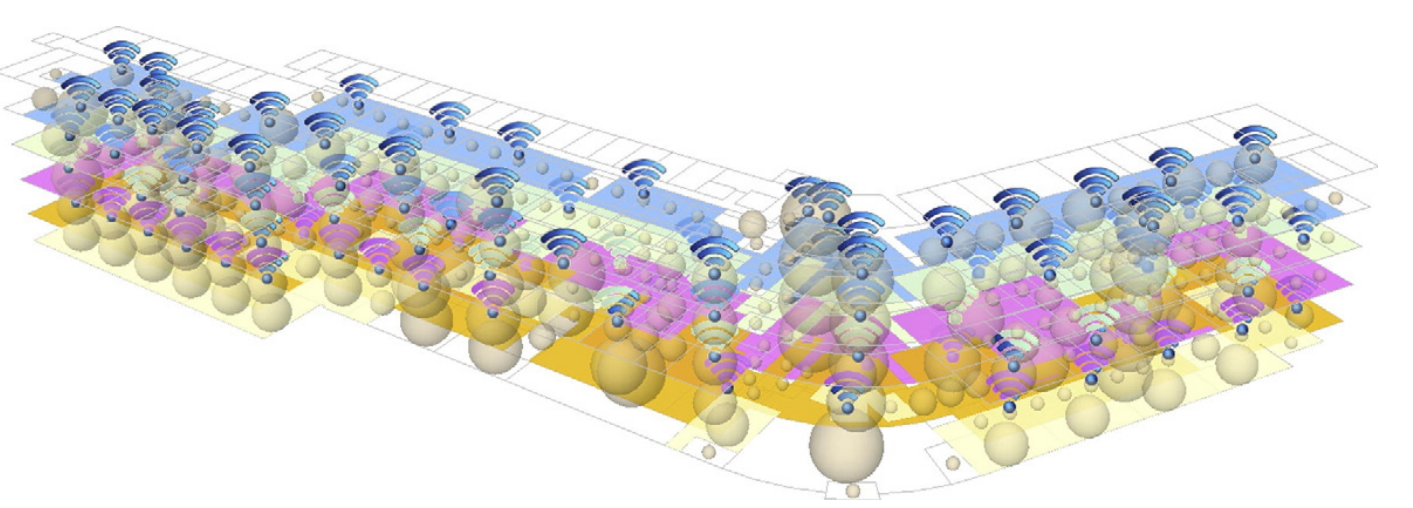
\includegraphics[width=1\textwidth]{2/figures/lee2015.png}
		\caption[Colocación óptima de AP capacitados con demandas ponderadas (p = 117)]{Colocación óptima de AP capacitados con demandas ponderadas (p = 117).\\
		Fuente: \cite{pr_lee2015coverage3d}. \citetitle{pr_lee2015coverage3d}. (p. 9)}
		\label{2:fig119}
	\end{center}
\end{figure}

\subsection{\citetitle{pr_ozerol2023genermass}}
En marzo de 2023, en la revista científica "Architecture and Planning Journal (APJ)", \cite{pr_ozerol2023genermass} publicaron el artículo conocido como \citetitle{pr_ozerol2023genermass}, en español, esto se traduce como "Creación de planes de vivienda colectiva a través de Gans - Un caso en Tokio, Turquía".

El estudio investigó la capacidad de Generative Adversarial Neural Networks (GAN) para crear dibujos arquitectónicos de proyectos de vivienda masiva de TOKI utilizando conjuntos de datos. El objetivo principal fue capacitar al algoritmo HouseGAN para crear tipologías de planos de TOKI actuales y diagramas de burbujas.

En el artículo se explica cómo se multiplicaron planos correlacionados espacialmente con la configuración RGB de 21 tipologías de planos para obtener 157 conjuntos de datos de planos. Estos datos se utilizaron para entrenar al algoritmo de deep learning HouseGAN, que generó imágenes de fondo realistas como salidas del proceso de entrenamiento. El estudio siguió los siguientes pasos: Los diseños arquitectónicos de los proyectos de vivienda masiva de TOKI se utilizaron como conjuntos de datos. Después, se multiplicaron los planos para obtener 157 conjuntos de datos de planos, que se correlacionaron espacialmente con la configuración RGB de 21 tipologías de planos. Posteriormente, se empleó el conjunto de datos generado para entrenar a HouseGAN. Finalmente, los resultados del entrenamiento se convirtieron en imágenes de fondo realistas.

La investigación reveló que la planificación del diseño espacial del algoritmo HouseGAN proporciona diagramas de burbujas y tipologías de planos de TOKI actuales. Como se muestra en la Figura 12, este método permitió crear planos arquitectónicos útiles y realistas para el desarrollo de proyectos de vivienda masiva.

\begin{figure}[!ht]
	\begin{center}
		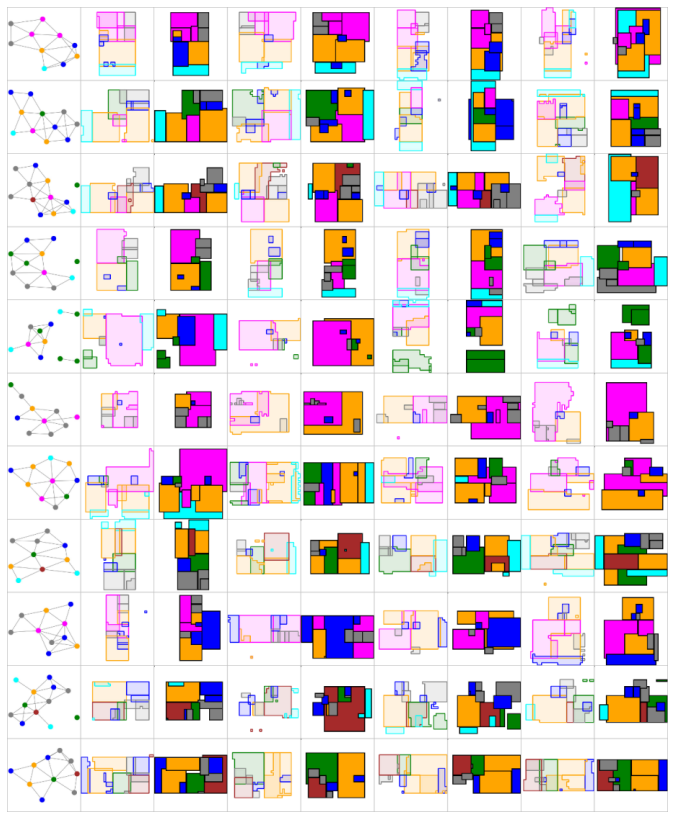
\includegraphics[width=1\textwidth]{2/figures/ozerol2023.png}
		\caption[HouseGAN con LIFULL HOMES Datasets, imágenes generadas por los autores]{HouseGAN con LIFULL HOMES Datasets, imágenes generadas por los autores.\\
		Fuente: \cite{pr_ozerol2023genermass}. \citetitle{pr_ozerol2023genermass}. (p. 10)}
		\label{2:fig120}
	\end{center}
\end{figure}

\subsection{\citetitle{pr_chang2021buildinggan}}
En abril del 2021, en la revista científica "arXiv", \cite{pr_chang2021buildinggan} publicaron el artículo conocido como \citetitle{pr_chang2021buildinggan}, el título "Building-GAN: generación de diseños arquitectónicos volumétricos condicionados por grafos" se traduce al español.

Se emplearon dos conjuntos de datos principales: uno propio de 157 planos de TOKI multiplicados espacialmente, y el conjunto de datos LIFULL HOMES utilizado por el algoritmo HouseGAN de fuente abierta. Para mejorar la eficiencia en el diseño volumétrico de edificios en la industria de la arquitectura y la construcción, este artículo presenta un enfoque innovador llamado Building-GAN. Para visualizar los diseños arquitectónicos, se introduce un grafo de voxels tridimensional, así como un generador que incorpora un módulo de punteros cruzados para conectar el grafo de programas y el grafo de voxels.

El artículo detalla los pasos que se deben seguir para crear el modelo Building-GAN. Comienza con la recopilación de datos, que produce un conjunto de datos sintéticos que incluye 120,000 diseños volumétricos de edificios comerciales. Luego se implementa un Grafo Neural Generativo (GNN) de voxels y se crea un grafo de programas jerárquico. Un módulo cruzado basado en punteros también se agrega para conectar los grafos de programas y los voxels.

Los resultados muestran que el modelo propuesto supera significativamente al método anterior, House-GAN, en un estudio de usuarios con 20 arquitectos profesionales, con una puntuación promedio de 0.85 y 0.92, respectivamente. Además, el modelo propuesto obtiene una puntuación promedio de 0.37 en comparación con el modelo Ground Truth, lo que indica que los arquitectos a menudo no pueden distinguir claramente entre el modelo Ground Truth y el modelo propuesto, como se muestra en la Figura 13.

\begin{figure}[!ht]
	\begin{center}
		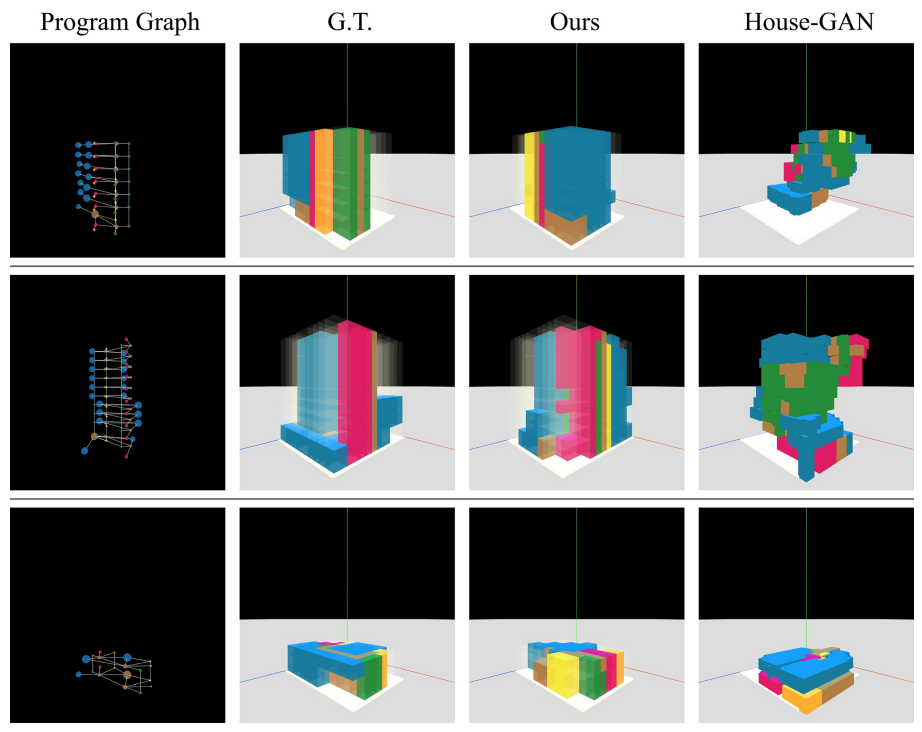
\includegraphics[width=0.7\textwidth]{2/figures/chang2021.png}
		\caption[Para cada gráfico de programa, se generan diseños volumétricos mediante nuestro modelo y mediante House-GAN]{Para cada gráfico de programa, se generan diseños volumétricos mediante nuestro modelo y mediante House-GAN.\\
		Fuente: \cite{pr_chang2021buildinggan}. \citetitle{pr_chang2021buildinggan}. (p. 7)}
		\label{2:fig121}
	\end{center}
\end{figure}

\subsection{\citetitle{pr_chen2020intelhome3d}}
\cite{pr_chen2020intelhome3d} publicaron un artículo que se llamaba \citetitle{pr_chen2020intelhome3d}, en español, se ha traducido como "Inteligente Casa 3D: Diseño automático de casas en 3D solo a partir de descripciones lingüísticas" para la revista científica "arXiv" en 2020.

Este artículo presenta un modelo generativo que utiliza descripciones lingüísticas para diseñar automáticamente planos de casas en tres dimensiones. Dos tareas principales componen el proceso: generar el plano de la planta y la síntesis de las texturas internas.

Los siguientes son los pasos que componen la metodología: representar las descripciones lingüísticas en un grafo estructural utilizando un analizador de escenas de Stanford, utilizando una red neuronal condicional de grafos (GC-LPN) para crear un diseño de planta grueso. Refinar el diseño grueso para crear un plano que incluya puertas y ventanas, Usando una red generativa adversaria condicional a lenguaje (LCT-GAN), se pueden sintetizar las texturas interiores de cada habitación. crear y mostrar la escena 3D completa a partir del plano con texturas.

Los hallazgos indican que el 39,41\% de los diseños creados por el modelo no se distinguían de los creados por humanos en un estudio en el que participaron 20 personas. Además, en evaluaciones cuantitativas, el modelo obtuvo un puntaje de IoU de 0,4765 para la generación de planos y un FID de 27,32 para la síntesis de texturas.

\begin{figure}[!ht]
	\begin{center}
		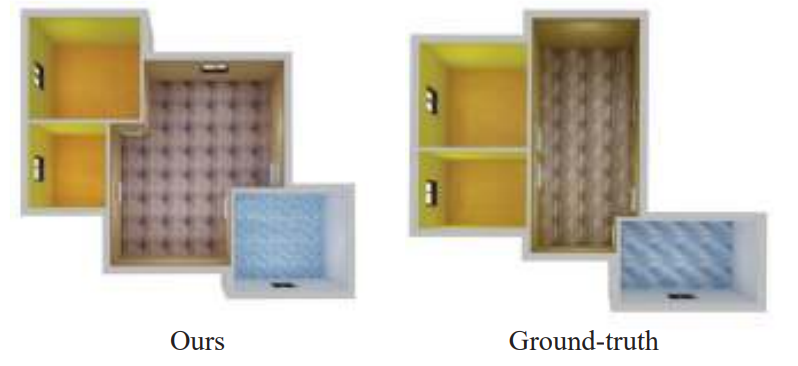
\includegraphics[width=0.73\textwidth]{2/figures/chen2020.png}
		\caption[Comparación de nuestros planos de casas en 3D generados con sus contrapartes reales (hechas por humanos)]{Comparación de nuestros planos de casas en 3D generados con sus contrapartes reales (hechas por humanos).\\
		Fuente: \cite{pr_chen2020intelhome3d}. \citetitle{pr_chen2020intelhome3d}. (p. 8)}
		\label{2:fig122}
	\end{center}
\end{figure}

\subsection{\citetitle{pr_dou2023researchwir}}
\cite{pr_dou2023researchwir} publicaron un artículo que se llamaba \citetitle{pr_dou2023researchwir}, "Investigación sobre cobertura de red inalámbrica para la transformación y actualización de la gestión expositiva con tecnología de inteligencia artificial", según la revista académica internacional "Matemáticas aplicadas y ciencias no lineales" en junio de 2023.

El rápido crecimiento de la inteligencia artificial y la tecnología de comunicación moderna ofrece una oportunidad poderosa para transformar, actualizar y desarrollar una gestión de exposiciones de alta calidad. Sin embargo, es necesario abordar el problema de la cobertura ideal de la red inalámbrica en el área de exposición. Se ha introducido un nuevo algoritmo de inteligencia artificial basado en la optimización de Harris Hawk (HHO) para abordar este problema.

El artículo resuelve el problema de cobertura de la red inalámbrica utilizando un método de optimización multiobjetivo. Primero, el problema de la cobertura se plantea como una función de objetivo que busca maximizar la cobertura y minimizar la redundancia. Como se muestra en la Figura 14, se resuelve este problema utilizando el algoritmo de optimización de Harris Hawk mejorado (IHHO). El IHHO permite una búsqueda eficiente del espacio de soluciones al simular el comportamiento de los halcones de Harris al cazar presas. Además, para inicializar la población, se utiliza un muestreo de hipercubo latino, lo que mejora la diversidad de la población inicial y reduce la probabilidad de convergencia prematura.

\begin{figure}[!ht]
	\begin{center}
		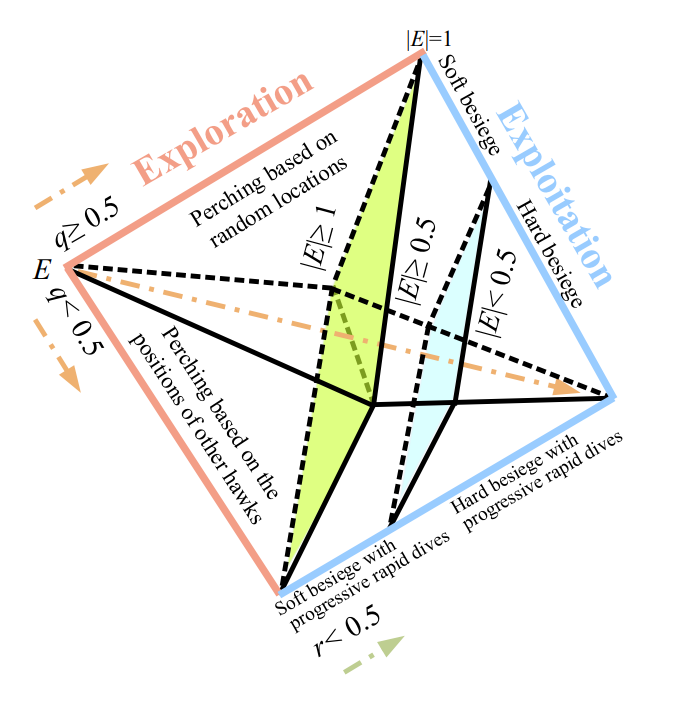
\includegraphics[width=0.5\textwidth]{2/figures/dou2023.png}
		\caption[Estructura de HHO]{Estructura de HHO.\\
		Fuente: \cite{pr_dou2023researchwir}. \citetitle{pr_dou2023researchwir}. (p. 5)}
		\label{2:fig123}
	\end{center}
\end{figure}

Como se muestra en la Figura 15, los resultados de la simulación muestran que el algoritmo de optimización tiene un índice de evaluación integral del 98,03\%, que es superior al del optimizador de enjambre de partículas (PSO) y al algoritmo HHO estándar. Esto demuestra que el algoritmo IHHO sugerido es efectivo para resolver los problemas de cobertura de la red inalámbrica y mejora la cobertura de los nodos más que los métodos de optimización convencionales.

\begin{figure}[!ht]
	\begin{center}
		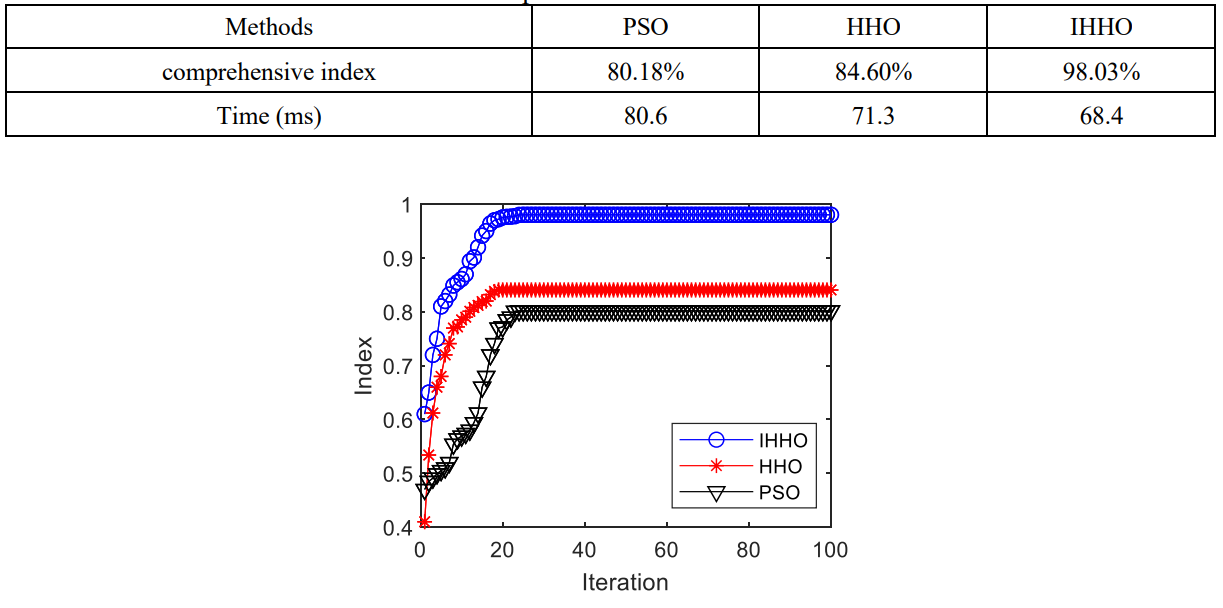
\includegraphics[width=0.5\textwidth]{2/figures/dou2023_2.png}
		\caption[Comparaciones entre los métodos]{Comparaciones entre los métodos.\\
			Fuente: \cite{pr_dou2023researchwir}. \citetitle{pr_dou2023researchwir}. (p. 11)}
		\label{2:fig124}
	\end{center}
\end{figure}
\clearpage